\documentclass[table,xcolor=table]{IFMG-beamer}

% --------------------------------------------------- %
%                  Informações      	              %
% --------------------------------------------------- %
\title[PSLG]{PSLG}
\subtitle{Week 07}
\author{Dawid Sobczak \& Tomasz Zajas }
% \institute[IFMG]{University of Limerick}
\date[\today]{}


\subject{Meu tema } % metadata

% --------------------------------------------------- %
%                    Title + Schedule                 %
% --------------------------------------------------- %

\begin{document}

\bgroup%
\setbeamertemplate{navigation symbols}{}
\makeatother
\bgroup%

\setbeamertemplate{footline}
{
  \leavevmode%
  \hbox{%
  \begin{beamercolorbox}[wd=.2\paperwidth,ht=2.25ex,dp=1ex,center]{author in head/foot}%
    \usebeamerfont{author in head/foot}\insertshortauthor%\expandafter\beamer\ifempty\expandafter{\beamer\shortinstitute}{}{~~(\insertshortinstitute)}
  \end{beamercolorbox}%
  \begin{beamercolorbox}[wd=.65\paperwidth,ht=2.25ex,dp=1ex,center]{title in head/foot}%
    \usebeamerfont{title in head/foot}\insertshorttitle%
  \end{beamercolorbox}%
  \begin{beamercolorbox}[wd=.15\paperwidth,ht=2.25ex,dp=1ex,center]{date in head/foot}%
    \usebeamerfont{date in head/foot}\insertshortdate{}%\hspace*{2em}
%    \insertframenumber{} / \inserttotalframenumber\hspace*{2ex} 
    %\hspace*{6ex}
  \end{beamercolorbox}}%
  \vskip0pt%
}


\begin{frame}
    \maketitle
\end{frame}


\egroup%

\setbeamertemplate{footline}
{
 \leavevmode%
  \hbox{%
  \begin{beamercolorbox}[wd=.2\paperwidth,ht=2.25ex,dp=1ex,center]{author in head/foot}%
    \usebeamerfont{author in head/foot} \insertshortauthor{}
  \end{beamercolorbox}%
  \begin{beamercolorbox}[wd=.65\paperwidth,ht=2.25ex,dp=1ex,center]{title in head/foot}%
    \usebeamerfont{title in head/foot}\insertshorttitle%
  \end{beamercolorbox}%
  \begin{beamercolorbox}[wd=.15\paperwidth,ht=2.25ex,dp=1ex,right]{date in head/foot}%
    %\usebeamerfont{date in head/foot}\insertshortdate{}\hspace*{2em}
    \insertframenumber{} %/ \inserttotalframenumber
    \hspace*{6ex}
  \end{beamercolorbox}}%
  \vskip0pt%
}

\setcounter{framenumber}{0}

\hyphenation{non-interpreted}

% ----------------------------------------- %

\section{Plan}

\begin{frame}{Plan}

  \begin{itemize}[<+->]
    \item Overview of stack /  queues / compilation.
    \item Demo of compilation.
    \item Do some lab questions / Cover any material ye need help with.
  \end{itemize}

\end{frame}

\section{Stacks and Queues}
\subsection{Queues}

\begin{frame}{Stack}
  \begin{figure}
    \centering
    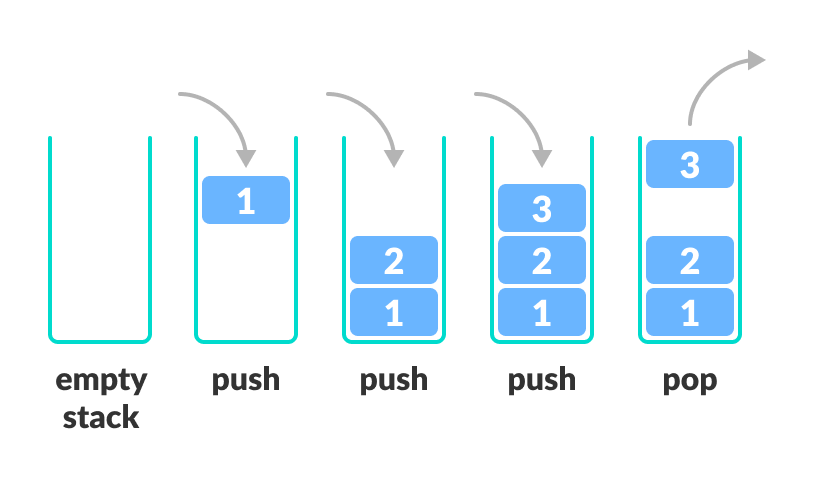
\includegraphics[width=0.8\linewidth]{figs/stack.png}
  \end{figure}
\end{frame}

\subsection{Stack}
\begin{frame}{Queue}
  \begin{figure}
    \centering
    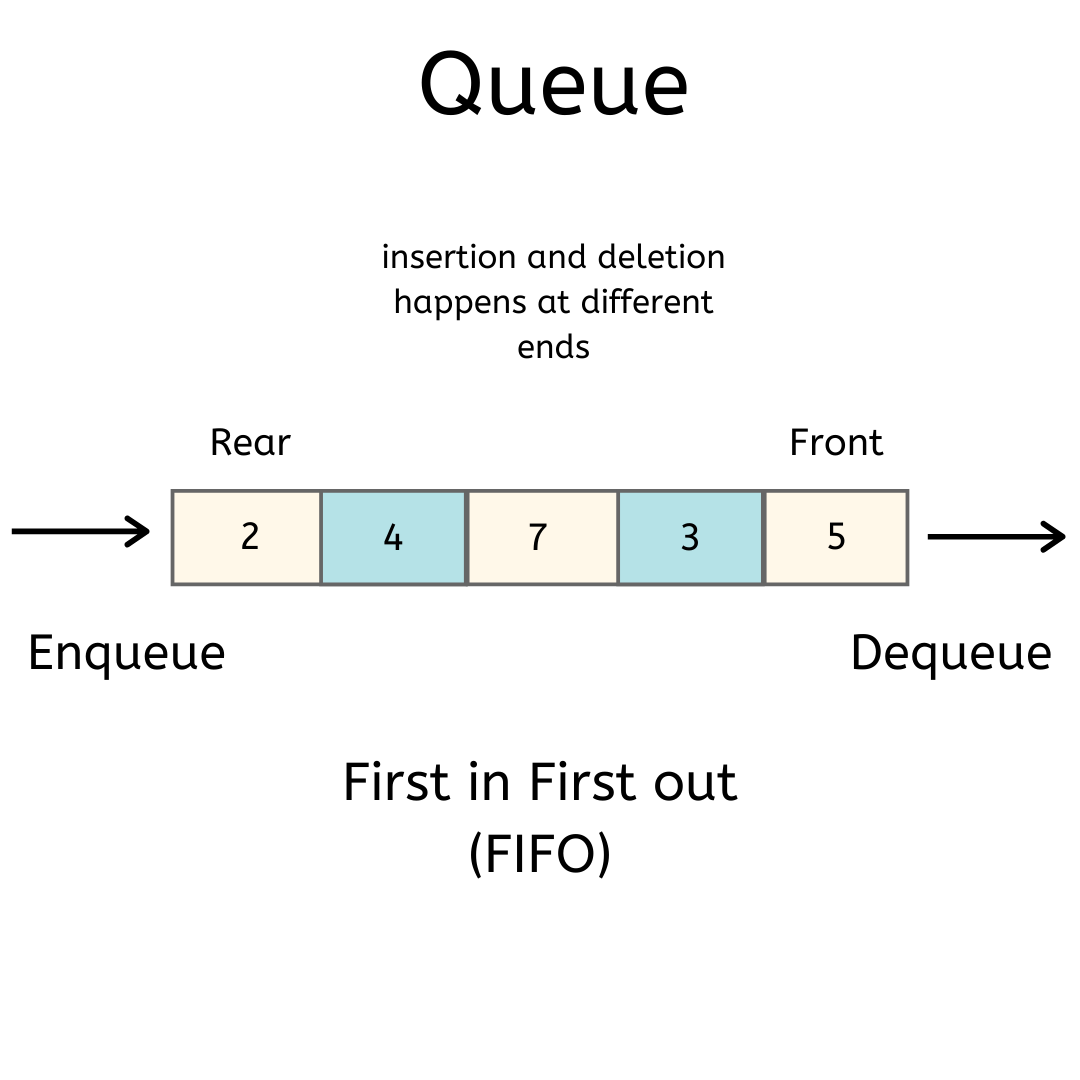
\includegraphics[width=0.8\linewidth]{figs/queue.png}
  \end{figure}
\end{frame}

\section{Compilation}
\subsection{What is compilation?}
\begin{frame}{Compilation in Java}
  \begin{itemize}
    \item Compiling code is the process of taking our programmer-readable ``source-code'' and converting it to ``executable code''.
    \item Our IDE (BlueJ) does this for us. Other IDE's do this too.
    \item This has allowed us to focus on Java's features and syntax.
  \end{itemize}
\end{frame}


\begin{frame}{Compilation in Java}

  \begin{itemize}[<+->]
    \item Java is both a compiled and an interpreted language.
    \begin{block}{``Interpreted''}
      \begin{itemize}
        \item In an \textbf{interpreted} language, the source code is read and executed by another program called an \textbf{interpreter} \\
        \item In a regular \textbf{non-interpreted} language, the source code is compiled directly into machine code that executes on the CPU. \\
      \end{itemize}
    \end{block}
    \begin{block}{``Compiled''}
      \begin{itemize}
        \item In a \textbf{compiled} language, the source code is transformed into another format that is more suitable to a particular task. 
        \item Java is compiled from its source code to bytecode so that the java virtual machine can execute it.  \\
      \end{itemize}
    \end{block}
  \end{itemize}

\end{frame}

\begin{frame}{Java Compilation}
  \begin{itemize}
    \item Java source code is first compiled into \textbf{bytecode}.
    \item This bytecode is then executed by the \textbf{Java Virtual Machine} (JVM).
  \end{itemize}

  \begin{block}{``Bytecode'' - Wikipedia Definition}
    \textit{Bytecode is a form of instruction set designed for efficient execution by a software interpreter}. Unlike human-readable source code, bytecodes are compact numeric codes, constants, and references (normally numeric addresses) that encode the result of compiler parsing and performing semantic analysis of things like type, scope, and nesting depths of program objects.
  \end{block}
\end{frame}

\subsection{Compilation Demo}
\begin{frame}{``Compilation Demo}
  \begin{block}{Java Hello World}
    \inputminted{C}{code/hello_world.java}
  \end{block}
\end{frame}

\end{document}
